
\chapter{Shallow water Acoustic Communication Channel Characterization}

\section{Stochastic Channel Model}
In many ways, shallow water acoustic communication channel resembles
an Ultra Wide Band(UWB) communication channel. Although its absolute
bandwidth is small ( usually less than 100k Hz), the relative
bandwidth, defined as the ratio of single sided bandwidth to the
carrier frequency, can be very large (typically greater than 20\%).
Just like a UWB channel, the shallow water acoustic communication
channel also shows a very strong tendency to clustering.
%\subsection{Modified Saleh-Valenzuela Model}

\subsection{Saleh-Valenzuela model and Modifications for Shallow
Water Channel}

Saleh-Valenzuela model and its modifications are a widely used
mathematic model for UWB channel. The classic Saleh-Valenzuela model
can be written as
\begin{equation}
h(t)=\sum_{l=0}^{L}\sum_{k=0}^{K}\alpha_{k,l}\exp(j\theta_{k,l})\delta(t-T_l-\tau_{k,l})
\end{equation}
where $\alpha_{k,l}$ is the magnitude of the $k$th component in the
$l$th cluster, $T_l$ is the arrival delay of the $l$th cluster,
$\tau_{k,l}$ is the delay of the $k$th component relative to the
beginning of  $l$th . We assume the phase $\theta_{k,l}$ is
uniformly distributed in the range of $[0, 2\pi]$. $K$ is the number
of components within a cluster. $L$ is the number of clusters.

The original SV model needs to be modified for Shallow Water
Channel. Depending on various factors like the channel geometry, the
environment, and the communication system, the number of clusters
$L$ is usually about 6-7, which includes all the detectable
clusters, but not all of them are significant for communication
purpose.

In some cases (like APL array), the rays with no surface interaction
showing little scattering effect, can be move from the summation,
\begin{equation}
h(t)=\alpha_D\delta(t-\tau_D)+\alpha_B\delta(t-\tau_B)+\sum_{l=1}^{L}\sum_{k=1}^{K}\alpha_{k,l}\exp(j\theta_{k,l})\delta(t-T_l-\tau_{k,l})
\end{equation}
where the $\alpha_D$ and $\alpha_B$ are the magnitudes for the
direct path and bottom path.


\subsection{Statistics of Group Energy}
 There have been lots of effort modeling the
amplitude of acoustic channel statistically, most of which were
focusing on the property and modeling of the amplitude as one random
variable. In previous sections, we already showed the group energy
of underwater acoustic channel has a strong correlation with surface
wave and wind condition, it becomes meaningful to inspect the
statistic property for each individual group. Unfortunately, there
were only about 60 transmissions in one packet, which isn't
statistically sufficient for a short geo time model. We have to turn
our attention to long geo time model.

Two distribution models are discussed in following subsections.
\subsubsection{Statistic model fitting}
\subsubsection*{ Rayleigh distribution}

Rayleigh distribution is given by

\begin{equation}
p(r)=\left\{ \begin{array}{ll}
         0 & \mbox{if $y < 0$};\\
        \frac{r}{\Omega}e^{\frac{-r^2}{2\Omega}} & \mbox{if $r \geq0$ }.\end{array}
        \right.
\end{equation}

Momentum stimulation is used to extract $\Omega$ parameter from
received data.
\subsection*{Log-normal distribution}
%y=1/(2*pi)^0.5/sigma./r.*exp(-(log(r)-nu).^2/2/sigma/sigma);
Log-normal distribution is :
\begin{equation}
p(r)=\frac{1}{\sqrt{2\pi}\sigma r}e^{(-\ln r
-\mu)^2/2\sigma^2}\end{equation}

$\mu$ and $\sigma$ can be estimated from data as
\begin{equation}
\mu =
\ln(\mathrm{E}(X))-\frac{1}{2}\ln\left(1+\frac{\mathrm{var}(X)}{\mathrm{E}(X)^2}\right)\end{equation}
\begin{equation}\sigma^2 =
\ln\left(1+\frac{\mathrm{var}(X)}{\mathrm{E}(X)^2}\right)\end{equation}


We found the log-normal distribution fits the data much better than
Rayleigh distribution.  The $\mu$ parameter keeps almost same for
different groups and does not change with the surface condition very
much. On the other hand, the $\sigma$ parameter has a strong
correlation with significant wave height.

\begin{figure}
\begin{center}
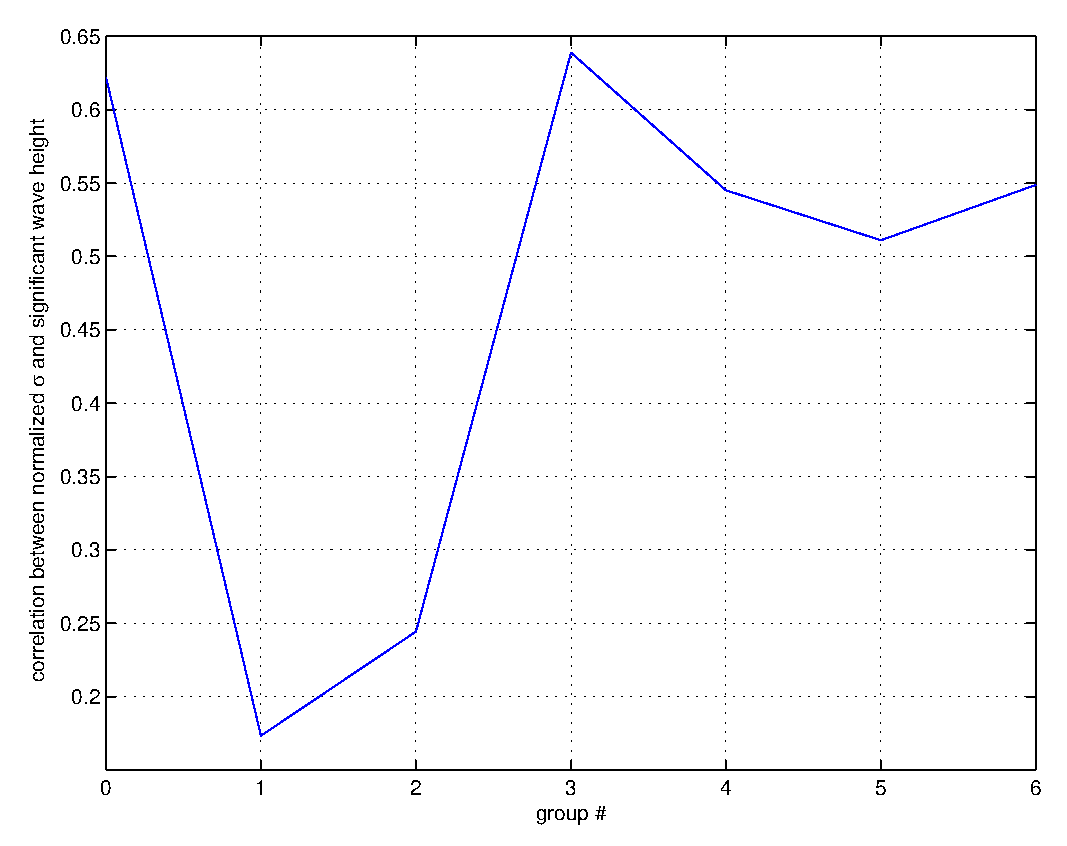
\includegraphics[width=3in]{correlation_sigma_waveheight.eps}
\caption{\normalsize correlatin between normalized $\sigma$ and
significant wave height }\label{fig-corr_sigma_wh}
\end{center}
\end{figure}

As expected, the group without surface interaction show little
correlation, while others show much stronger correlation between
$\sigma$ and significant wave height.
\subsection{Correlation with Environment Parameters}
\subsubsection{Correlation with water column variability}
The arrival time difference between direct path (group1) and
bottom-bounce path(group2) is shown in Fig.\ref{fig-directbottom}.
It's also possible to calculate the difference using ray tracing
model and the measurement of temperature from experiment. The result
is shown in Fig.\ref{fig-directbottom_bellhop}.
\subsubsection{Correlation with sea-surface condition}
To quantify the relation between the energy fluctuation in the
surface bounced paths and the surface wave, the normalized energy of
the two surface bounced paths is defined as $e_n=\frac{e-{\bf
E}\{e\}}{{\bf Std}\{e\}}$ with $e$ as energy of the two surface
bounced paths. From the acoustic data obtained from the APL array,
the cross-correlation between the normalized surface wave height and
the normalized energy is 0.9. Such strong correlation is shown in
Fig. \ref{fig-wave}(c). In other words, the energy of the surface
bounced paths decreases with the increase of the significant surface
wave height.

In Fig.\ref{fig-ge0} - \ref{fig-ge6} shows the normalized energy of
each group versus geo time. The normalized wind speed is also
plotted, which is defined as $ws_n=-\frac{ws-{\bf E}\{ws\}}{{\bf
Std}\{ws\}}$. The minus sign for the definition of $e_n$ is for
visualizing the correlation between $e_n$ and $ws_n$. $ws_n$ has a
clear trend that slowly decrease from the begin till July 2nd, 00:00
local time, after that, it starts climbing till the end of period.
Examining the energy of all 7 groups, group 0 (ambient noise) shows
a weak similarity with $ws_n$. group 3-6 (surface bouncing groups)
show some very strong similarity, but group 1,2 (direct and bottom
bouncing groups, with no surface interaction) show little
similarity. This is shown very clear when the correlation between
wind speed and group energy in Fig.\ref{fig-corr_w}. The maximum
correlation is group \#3, which is the group with one surface
interaction. It is also interesting that the correlation of surface
interacted groups(3,4,5,6) have a roughly decreasing trend. This
could be due to fact that each time of scattering (surface/bottom)
adds more smear onto the signal.
\begin{figure}
\begin{center}
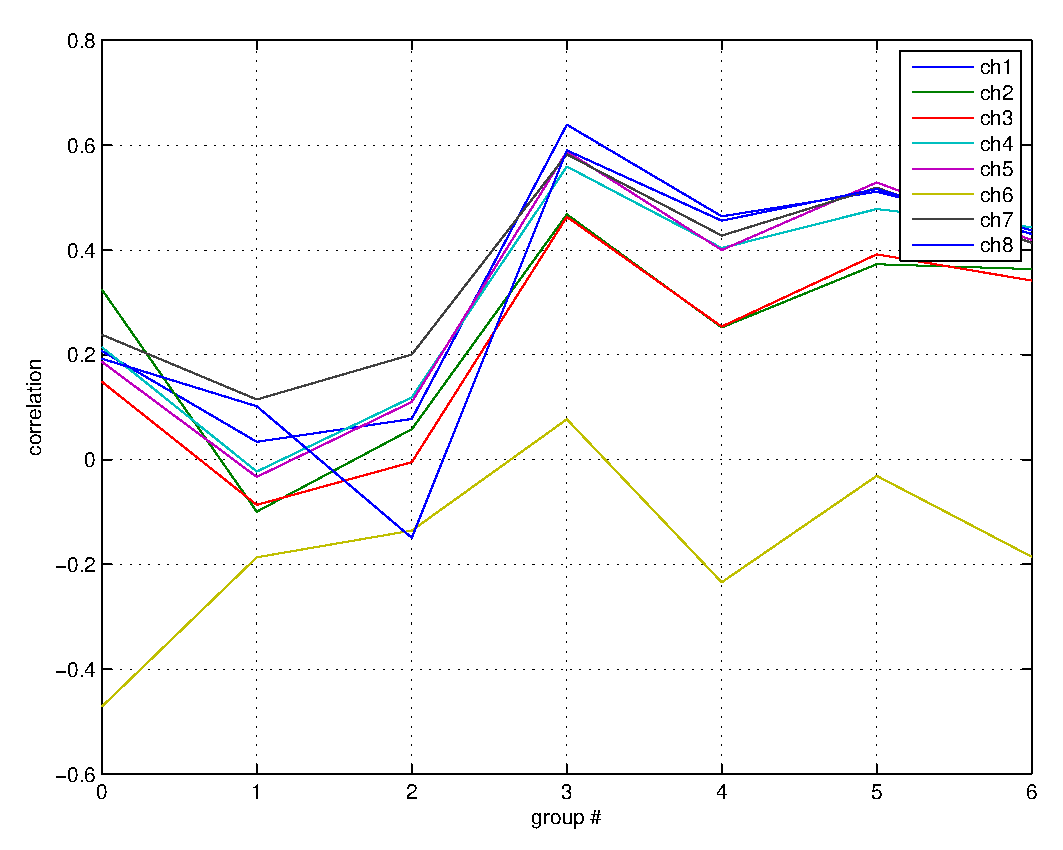
\includegraphics[width=3in]{correlation_energy_wind.eps}
\caption{\normalsize correlation between normalized group energy and
wind speed }\label{fig-corr_w}
\end{center}
\end{figure}

\begin{figure}
\begin{center}
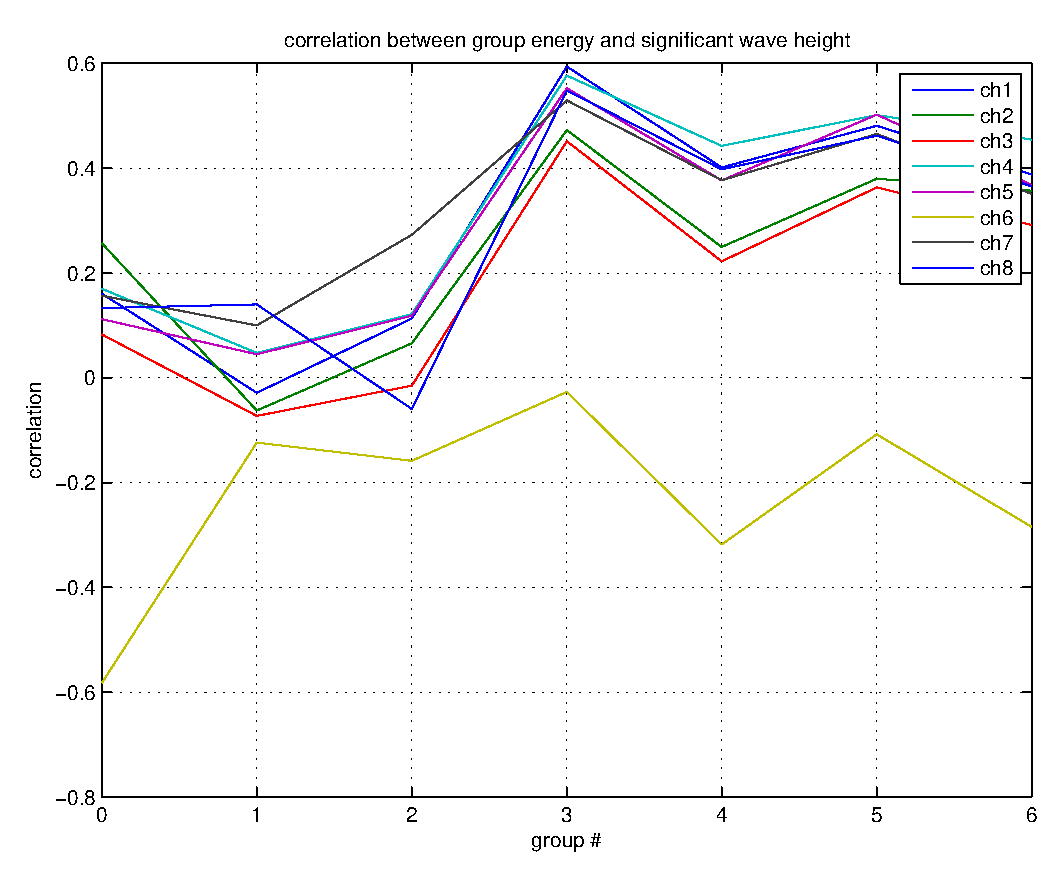
\includegraphics[width=3in]{correlation_energy_waveheight_1.eps}
\caption{\normalsize correlation between normalized group energy and
significant wave height }\label{fig-corr_h}
\end{center}
\end{figure}


It is well known the surface wave condition and wind speed have a
strong relationship. Therefore, it is little surprising when a
correlation between normalized significant wave height and
normalized group energy was found similar to the one between wind
speed and group energy. The result is shown in Fig.\ref{fig-corr_h}.
Just like the one in Fig.\ref{fig-corr_w}, the groups with no
surface interaction have little correlation with the significant
surface wave height, while the ones with surface interaction show a
strong correlation with it.

 The relation between
the normalized surface wave height and the normalized energy
fluctuation in the surface bounced paths leads to a possible way to
measure sea surface waves using acoustic measurement. At the same
time, such knowledge might lead to an interesting implication to
various Sonar applications such as underwater acoustic
communications: at calm sea condition, the channel seems to have
high signal-to-noise ratio (SNR) because the hydrophone will receive
higher energy through surface bounced paths. However, does this
mean, at calmer sea condition, the channel is more amicable to the
communication applications? To answer this question, the transmitted
communication signals have to be analyzed to investigate the
coherence of the channel impulse response function.


\subsection{Statistics of Decaying Rate}
\subsection{Statistics of Arrival Delay}



\subsection{Random Channel Realization}
